\apendice{Documentación de usuario}

\section{Introducción}
En esta sección se detalla como instalar y usar  la aplicación en un dispositivo Android.

\section{Requisitos de usuarios}

Los requisitos necesarios para poder ejecutar la aplicación son : 

\begin{itemize}
 	\item Disponer de una version de Android 5.0 Lollipop o superior.
 	\item Tener activado la instalación de Aplicaciones de orígenes desconocidos\cite{origenesDesconocidos}.
\end{itemize}

Para comprobar la versión de Android debemos ir a \textbf{Ajustes del dispositivo - Acerca del dispositivo  - Versión de Android}.

Para activar la opción de Orígenes desconocidos ir a \textbf{Ajustes del dispositivo - Seguridad  - Orígenes desconocidos}.

\section{Instalación}
Para instalar la aplicación en el dispositivo se debe instalar un fichero .apk\cite{apk}. Este fichero se puede obtener del CD que se adjunta en con la documentación, para ello es necesario trasferirlo al dispositivo y ejecutarlo. Si se tiene alguna duda de como trasferir datos del ordenador al dispositivo se recomienda consultar el enlace.
\begin{center}
	\url{https://support.google.com/nexus/answer/2840804?hl=es} 
\end{center}

El fichero apk también puede descargarse de la siguiente ruta.
\begin{center}
	\url{https://mega.nz/#F!cFBzwa7Z!78MPUPyZT0NyCwD1sEhX7Q}
\end{center}

Una vez el fichero se encuentra en el dispositivo, abrir este ejecutando un explorador de archivos y comenzará la instalación de la aplicación(ver figuras \ref{fig:instalacion1} y \ref{fig:instalacion2}).
\begin{figure}[ht]
		\centering
		\begin{minipage}[b]{0.45\linewidth}
			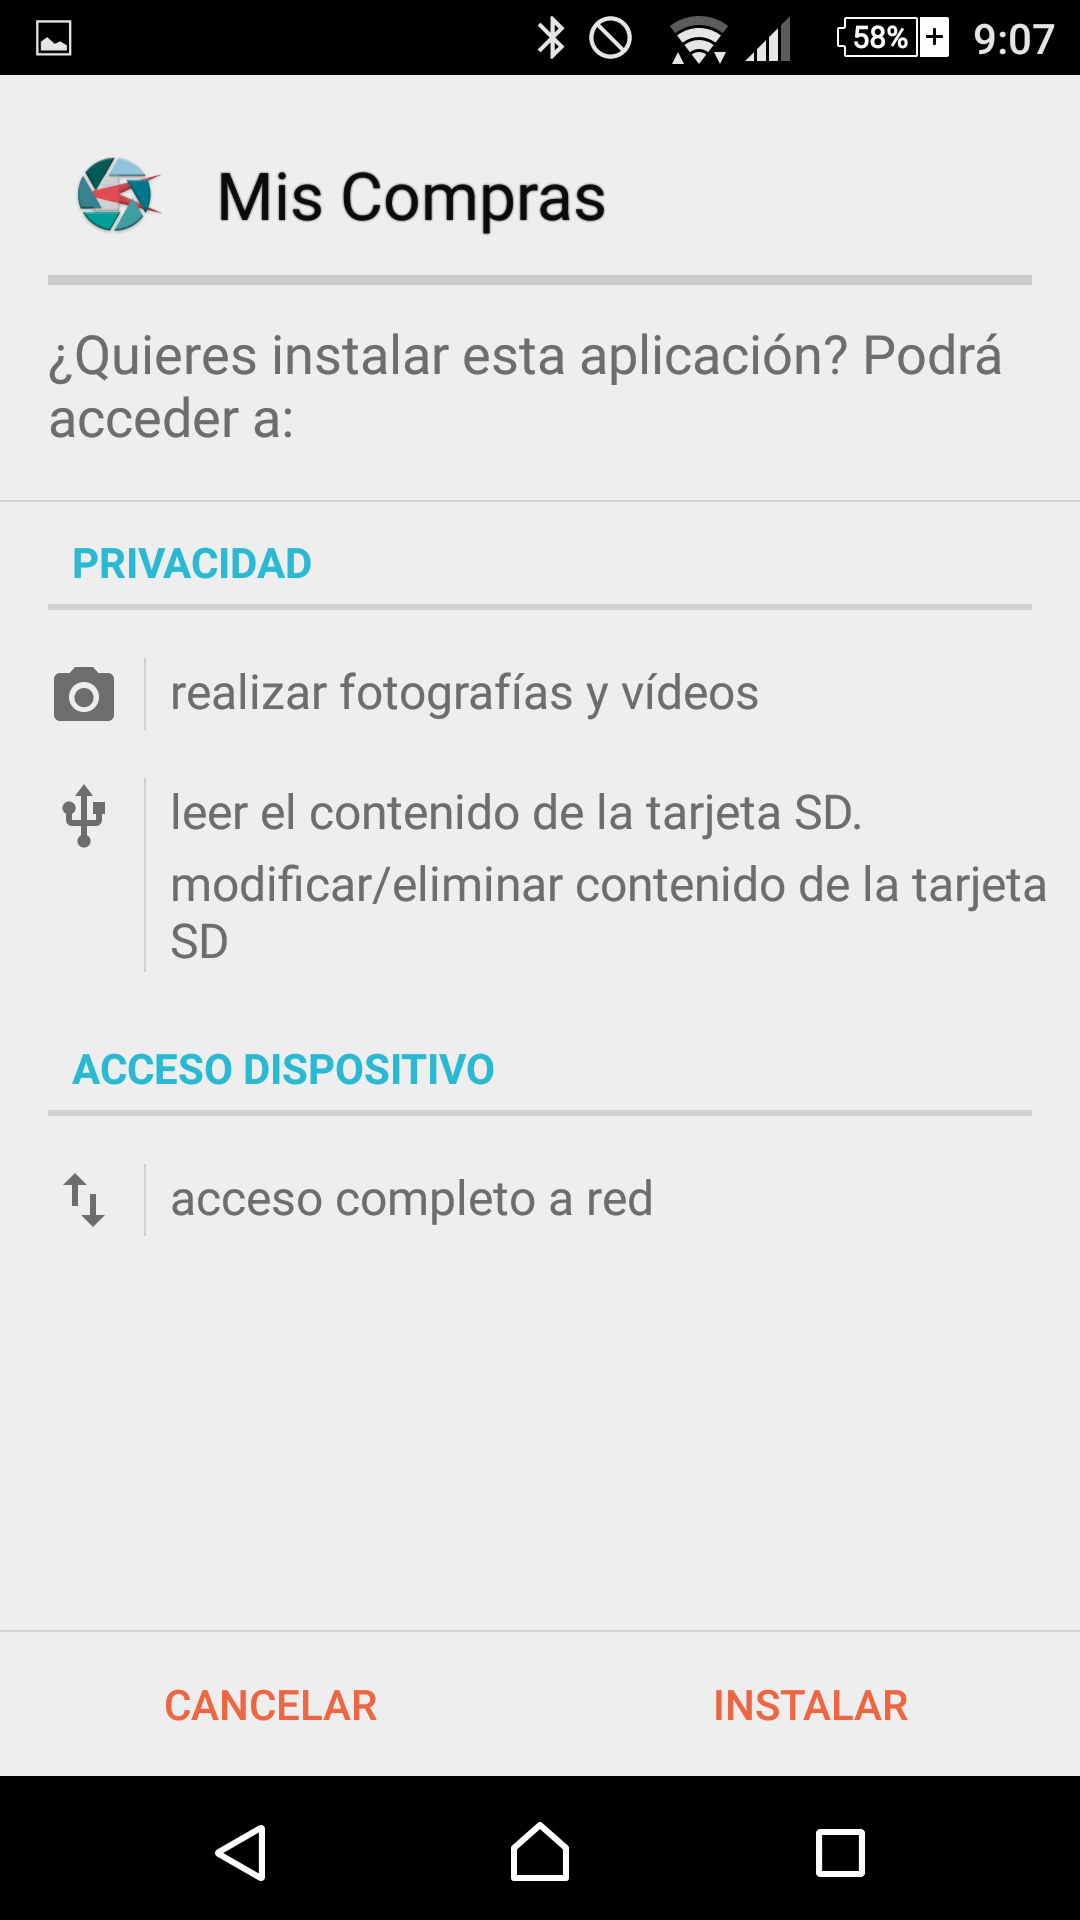
\includegraphics[width=\linewidth]{instalacion1.png}
			\caption{Paso de Instalación 1}
			\label{fig:instalacion1}
	\end{minipage}
	\quad
	\begin{minipage}[b]{0.45\linewidth}
		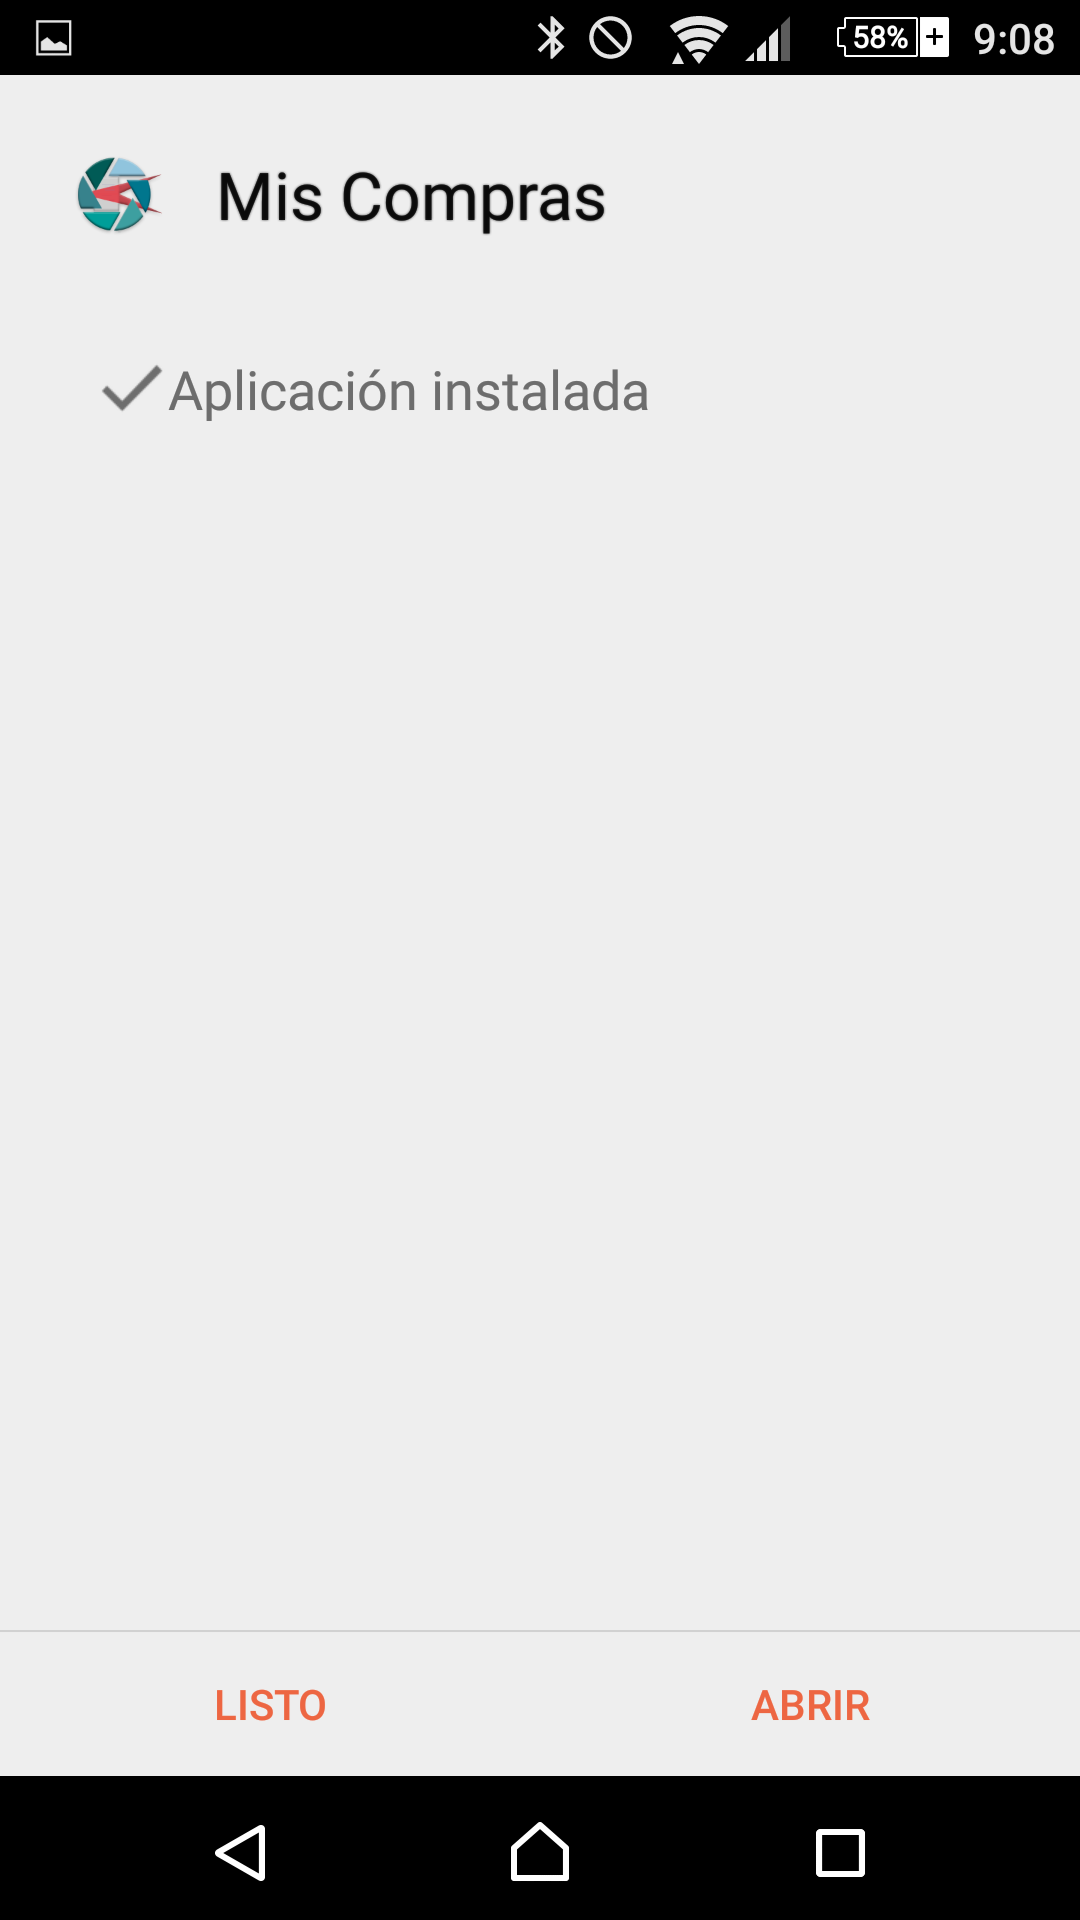
\includegraphics[width=\linewidth]{instalacion2.png}
		\caption{Paso de Instalación 2}
		\label{fig:instalacion2}
		\end{minipage}
	\end{figure}

\cleardoublepage
\section{Manual del usuario}

En esta sección se describe el uso de la aplicación.

\subsection{Menú de opciones de la aplicación. \label{menu}}

El menú de opciones de la aplicación se despliega deslizando el dedo desde el margen izquierdo de la pantalla hacia la derecha.

\begin{figure}[ht]
\begin{center}
\minipage{0.60\textwidth}
  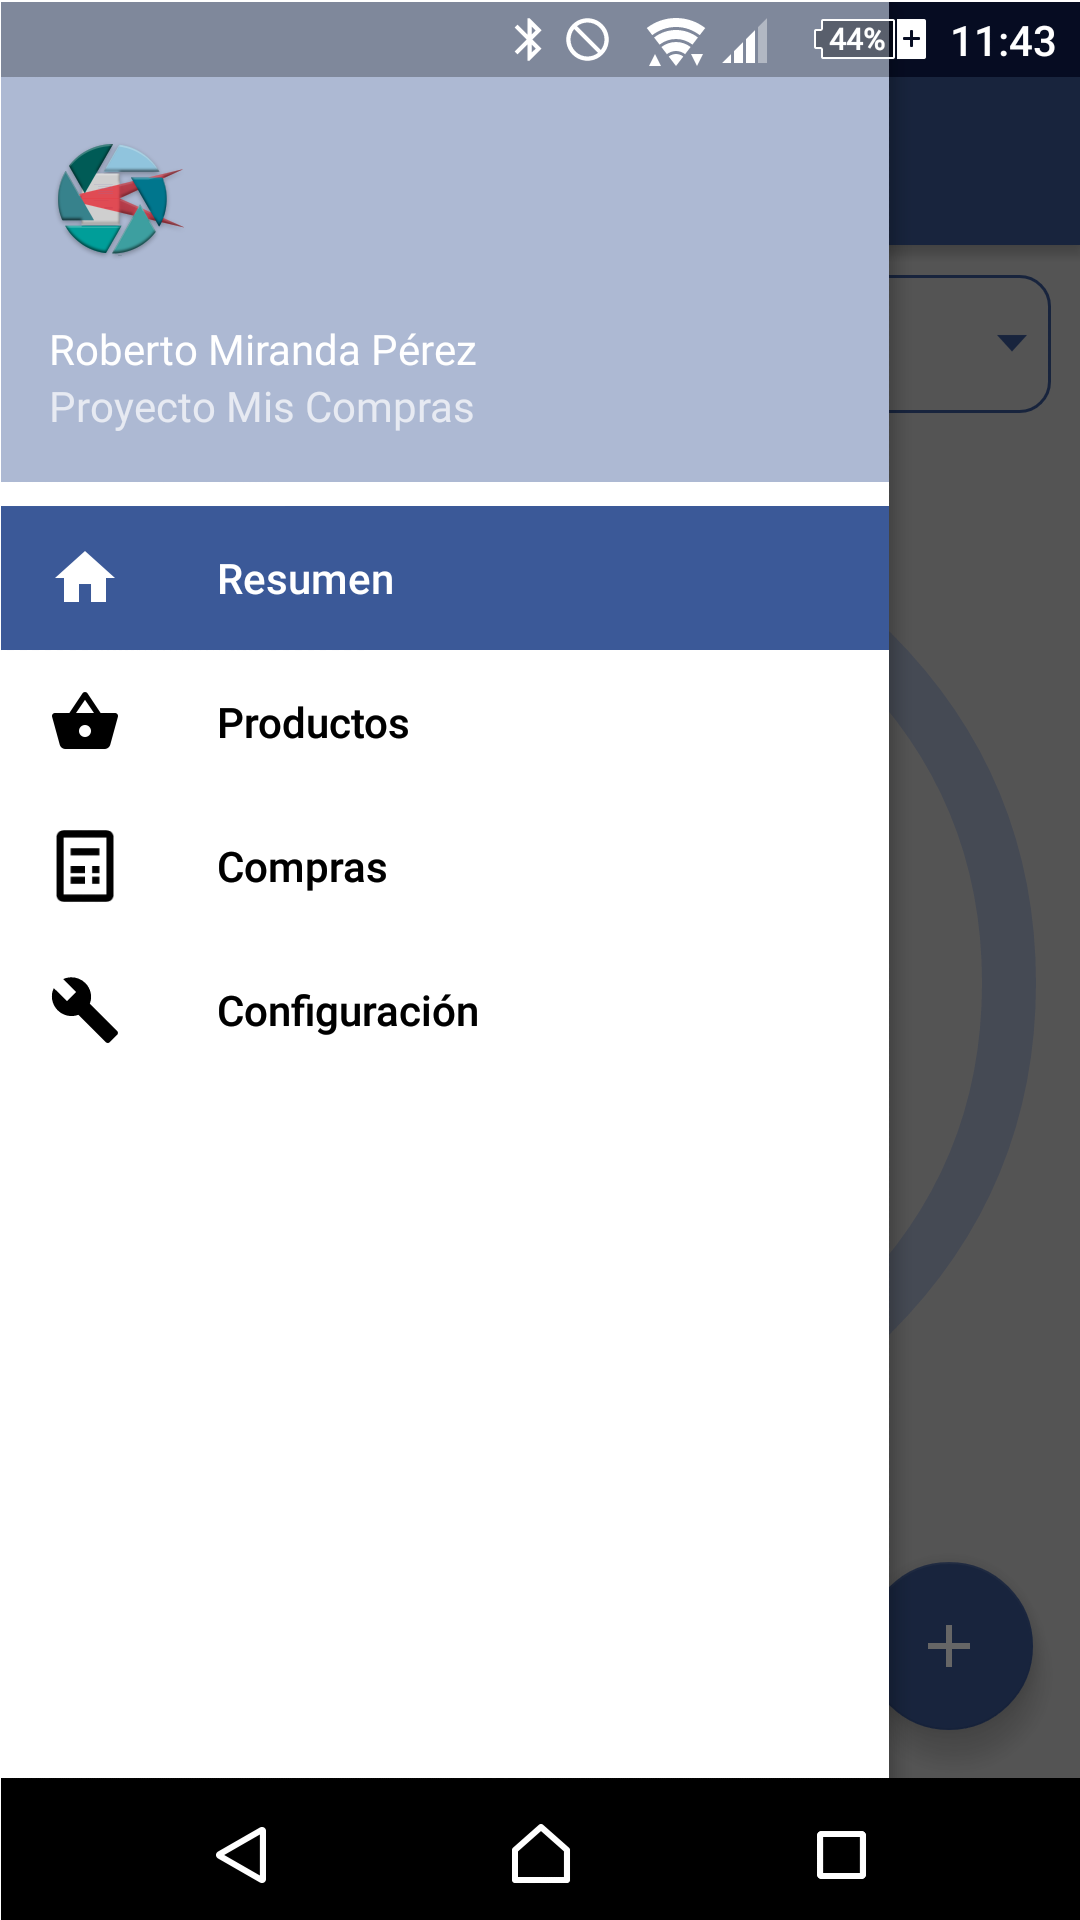
\includegraphics[width=\linewidth]{menu2.png}
  \caption{Menú de la aplicación.}\label{fig:menu}
\endminipage 
\end{center}
\end{figure}


Este menú consta de cuatro opciones que realizan diferentes funciones:
\begin{enumerate}
	\item \textbf{Resumen: }En esta pantalla se muestra un resumen de los gastos del usuario en un gráfico. Se visualiza el importe gastado por categoría y el porcentaje sobre el gasto total. También tiene la opción principal de añadir nuevos tiques (ver sección \ref{resumen} y \ref{nuevosTiques}).
	\item \textbf{Productos: }En esta pantalla se pueden consultar los productos adquiridos, permitiendo cambiar una serie de filtros para su búsqueda(ver sección \ref{consultaProdutos}).
	\item \textbf{Compras: }En esta pantalla se pueden consultar las compras realizadas, permitiendo cambiar una serie de filtros para su búsqueda(ver sección \ref{consultaCompras}).
	\item \textbf{Configuración: } Permite cambiar la dirección ip del servidor. 
\end{enumerate}


\subsection{Añadir Nuevo tique.\label{nuevosTiques}}
 Para empezar a usar la aplicación, pulse en el botón \ref{fig:boton1}
 para añadir una nueva imagen de tique. Este botón permite seleccionar el origen de la imagen que se desea cargar:
 \begin{itemize}
 	\item Botón \ref{fig:boton2} para cargar desde la galería.
 	\item Botón \ref{fig:boton3} para cargar desde la cámara.
 \end{itemize}
 \begin{figure}[!htb] 
\minipage{0.32\textwidth}
  
\includegraphics[width=\linewidth]{boton1.png}
  \caption{Añadir nueva imagen}\label{fig:boton1}
\endminipage\hfill
\minipage{0.32\textwidth}
  
\includegraphics[width=\linewidth]{boton2.png}
  \caption{Imagen de galeria}\label{fig:boton2}
\endminipage\hfill
\minipage{0.32\textwidth}%
  
\includegraphics[width=\linewidth]{boton3.png}
  \caption{Imagen de camara}\label{fig:boton3}
\endminipage
\end{figure}

Una ver seleccionada la imagen, seleccione el área del tique donde se encuentran los productos adquiridos utilizando el cuadro que se muestra encima de la imagen (ver figura \ref{fig:cargaImagen} , y pulse \textbf{Recortar} para empezar el proceso. Si desea cargar una imagen distinta, pulse en el botón \textbf{Cancelar}. 
\begin{figure}[ht]
\begin{center}
\minipage{0.60\textwidth}
  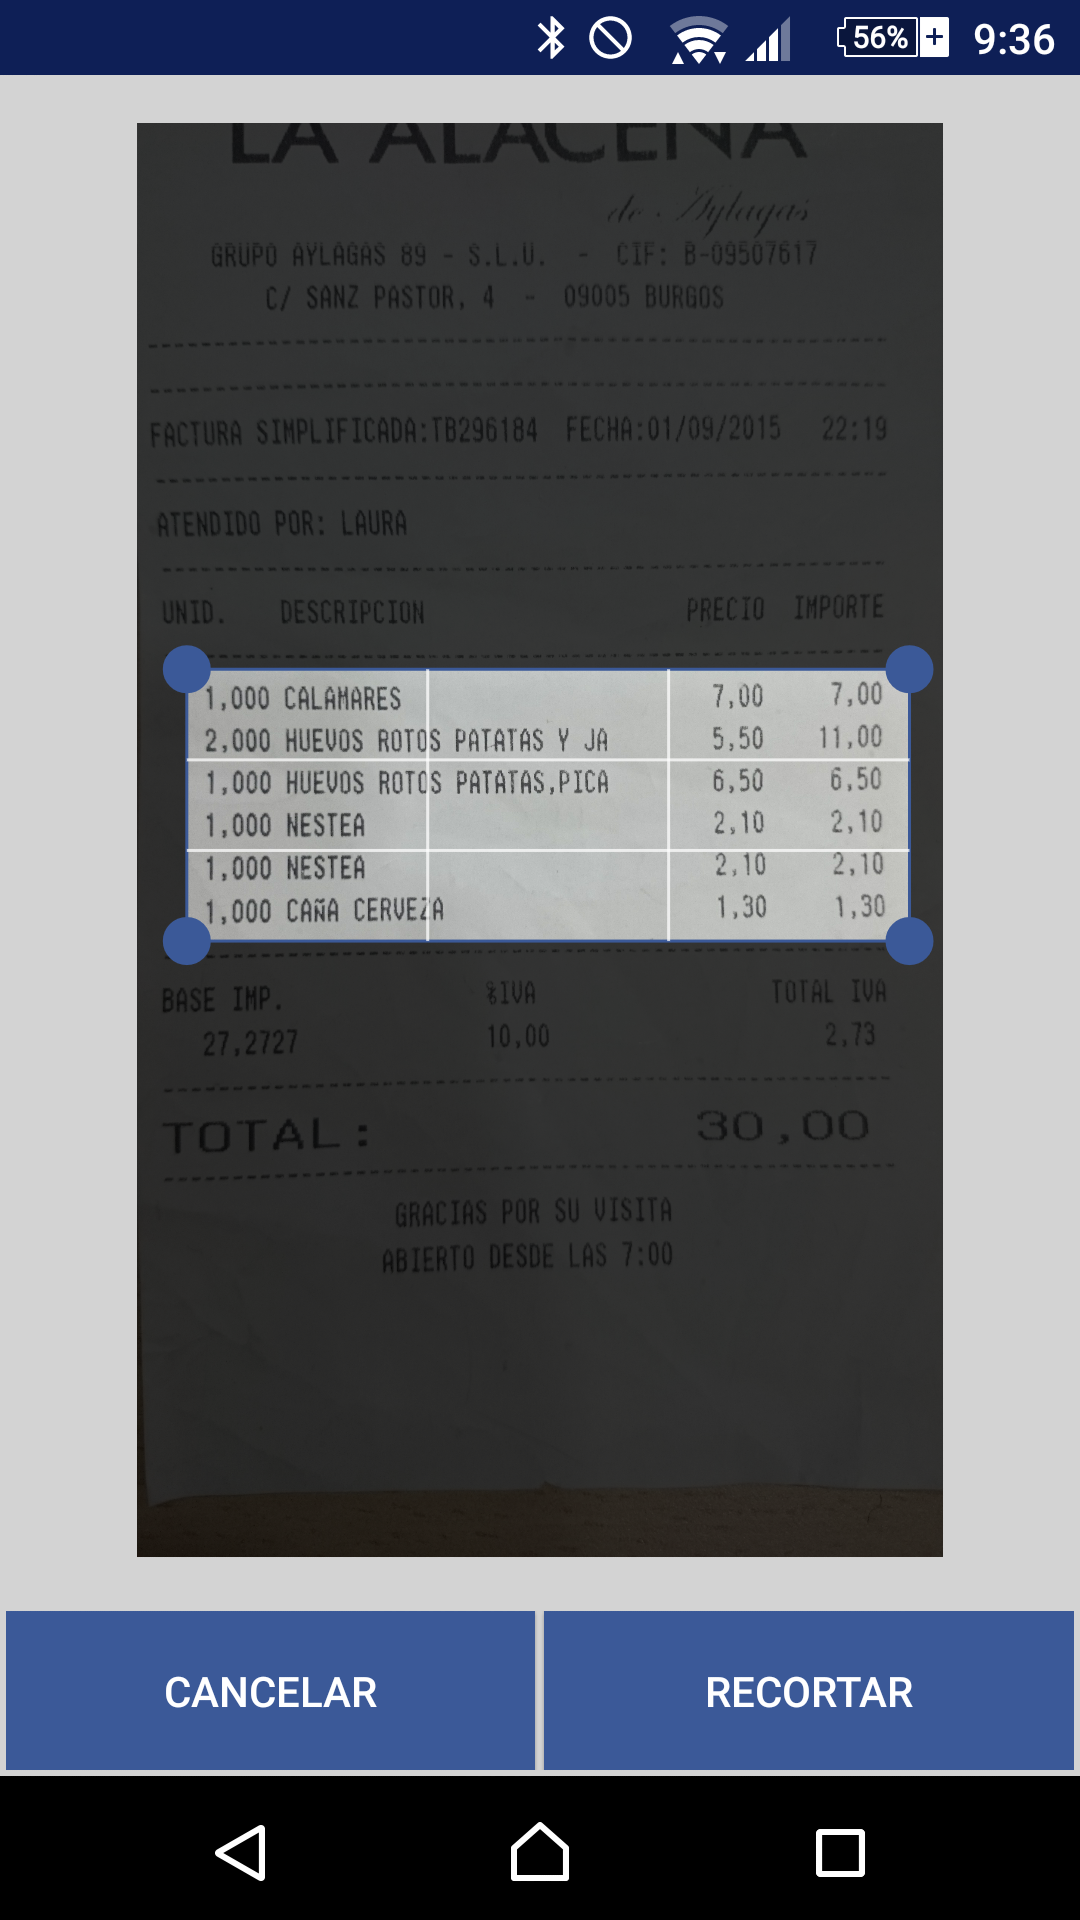
\includegraphics[width=\linewidth]{cargaImagen.png}
  \caption{Proceso de carga de nuevo tique.}\label{fig:cargaImagen}
\endminipage 
\end{center}
\end{figure}

Cuando empieza el proceso de carga de la imagen, se muestra un diálogo de progreso(ver figura \ref{fig:subida}), que una vez terminado si la imagen se ha procesado correctamente permitirá editar los elementos, sin embargo si hay algún error durante el proceso o conversión de la imagen, se mostrara un mensaje de error en la pantalla.
\imagen{subida}{Diálogo de subida}

Completado este proceso, se visualiza en formato de lista los elementos obtenidos(ver figura \ref{fig:cargaProductos}), si hay algún error de conversión el importe del producto se muestra en rojo, por el contrario si todo ha ido bien el color será verde.
En la cabecera del tique se detalla la fecha y el importe total de la compra.

Para poder editar un producto (cantidad, nombre, precio y categoría), se debe pulsar sobre el elemento que se quiere modificar, que abrirá un diálogo de edición. En este, se deben colocar los nuevos valores que se quieren para el producto(ver figura \ref{fig:dialogoEdicion}).

\begin{figure}[ht]
\minipage{0.45\textwidth}
  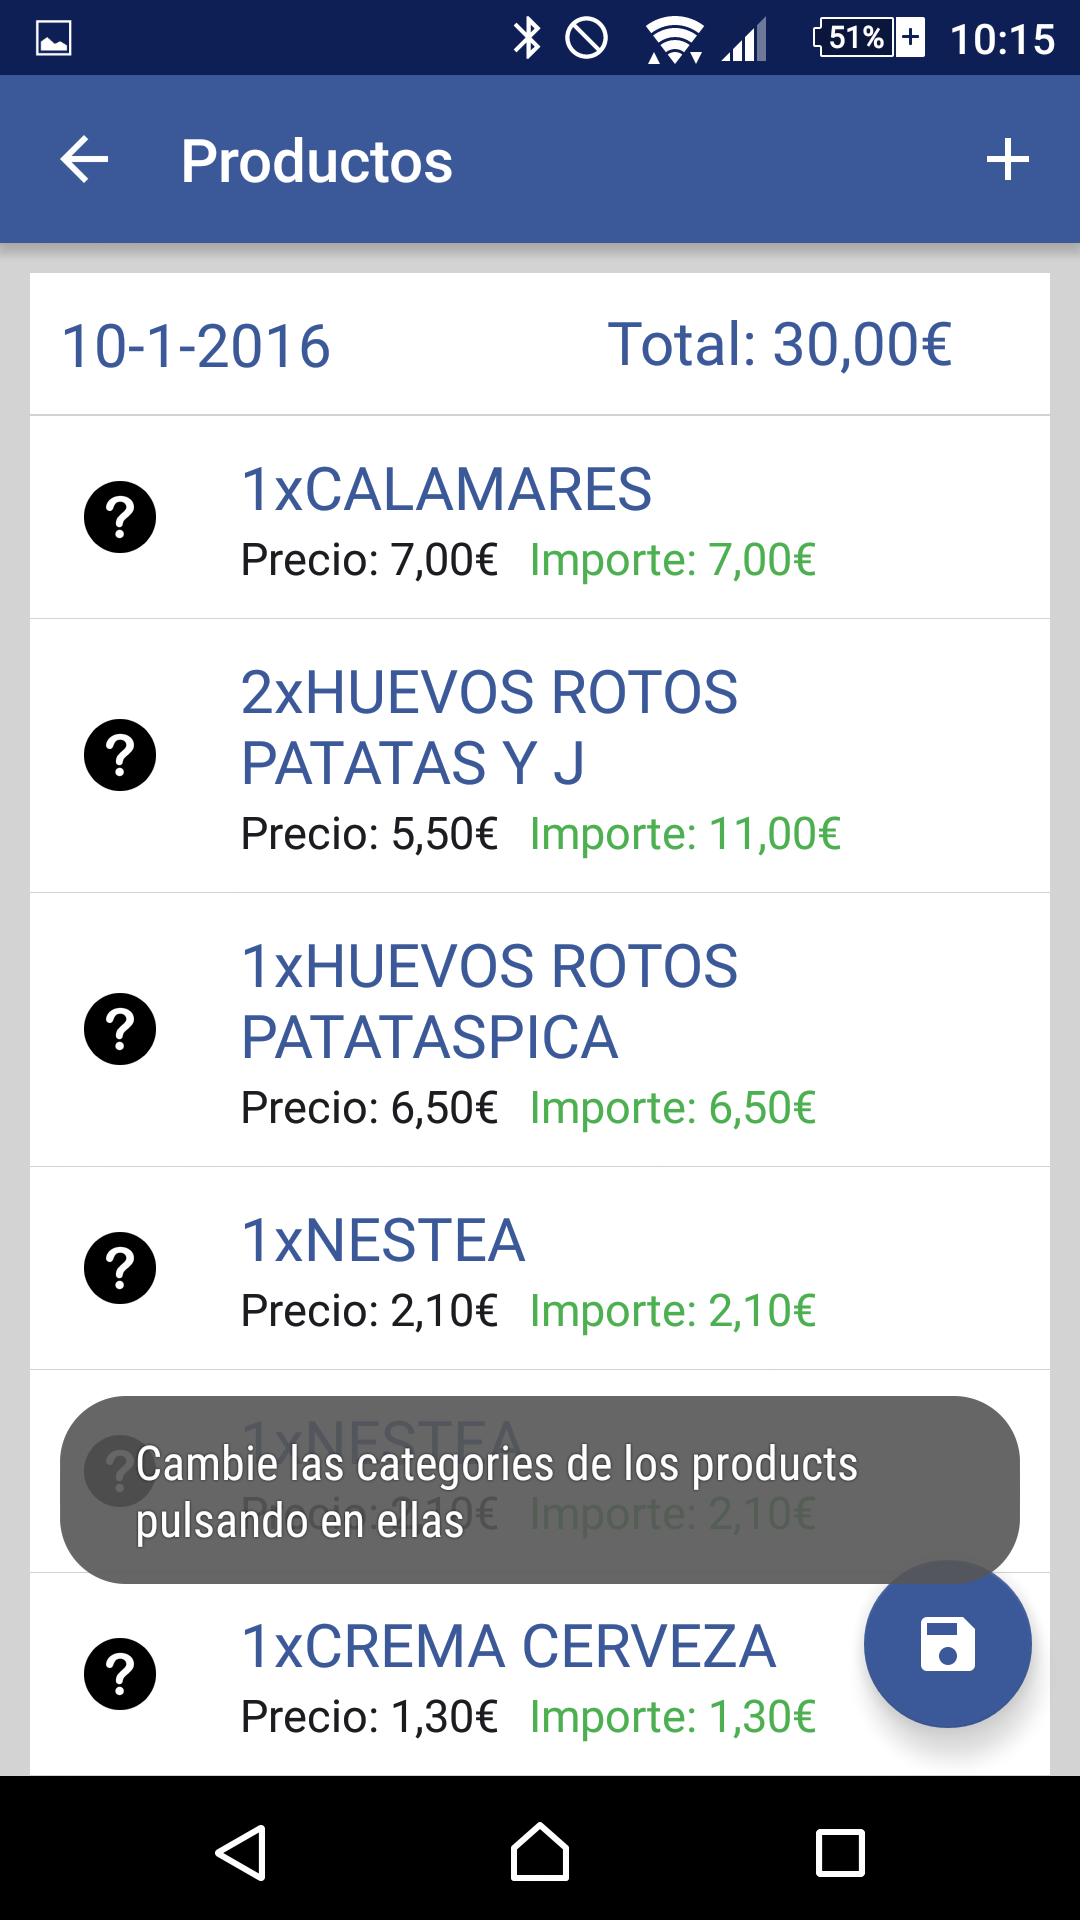
\includegraphics[width=\linewidth]{cargaProductos.png}ieren para el producto
  \caption{Carga de nuevos productos.}\label{fig:cargaProductos}
\endminipage\hfill
\minipage{0.45\textwidth}
  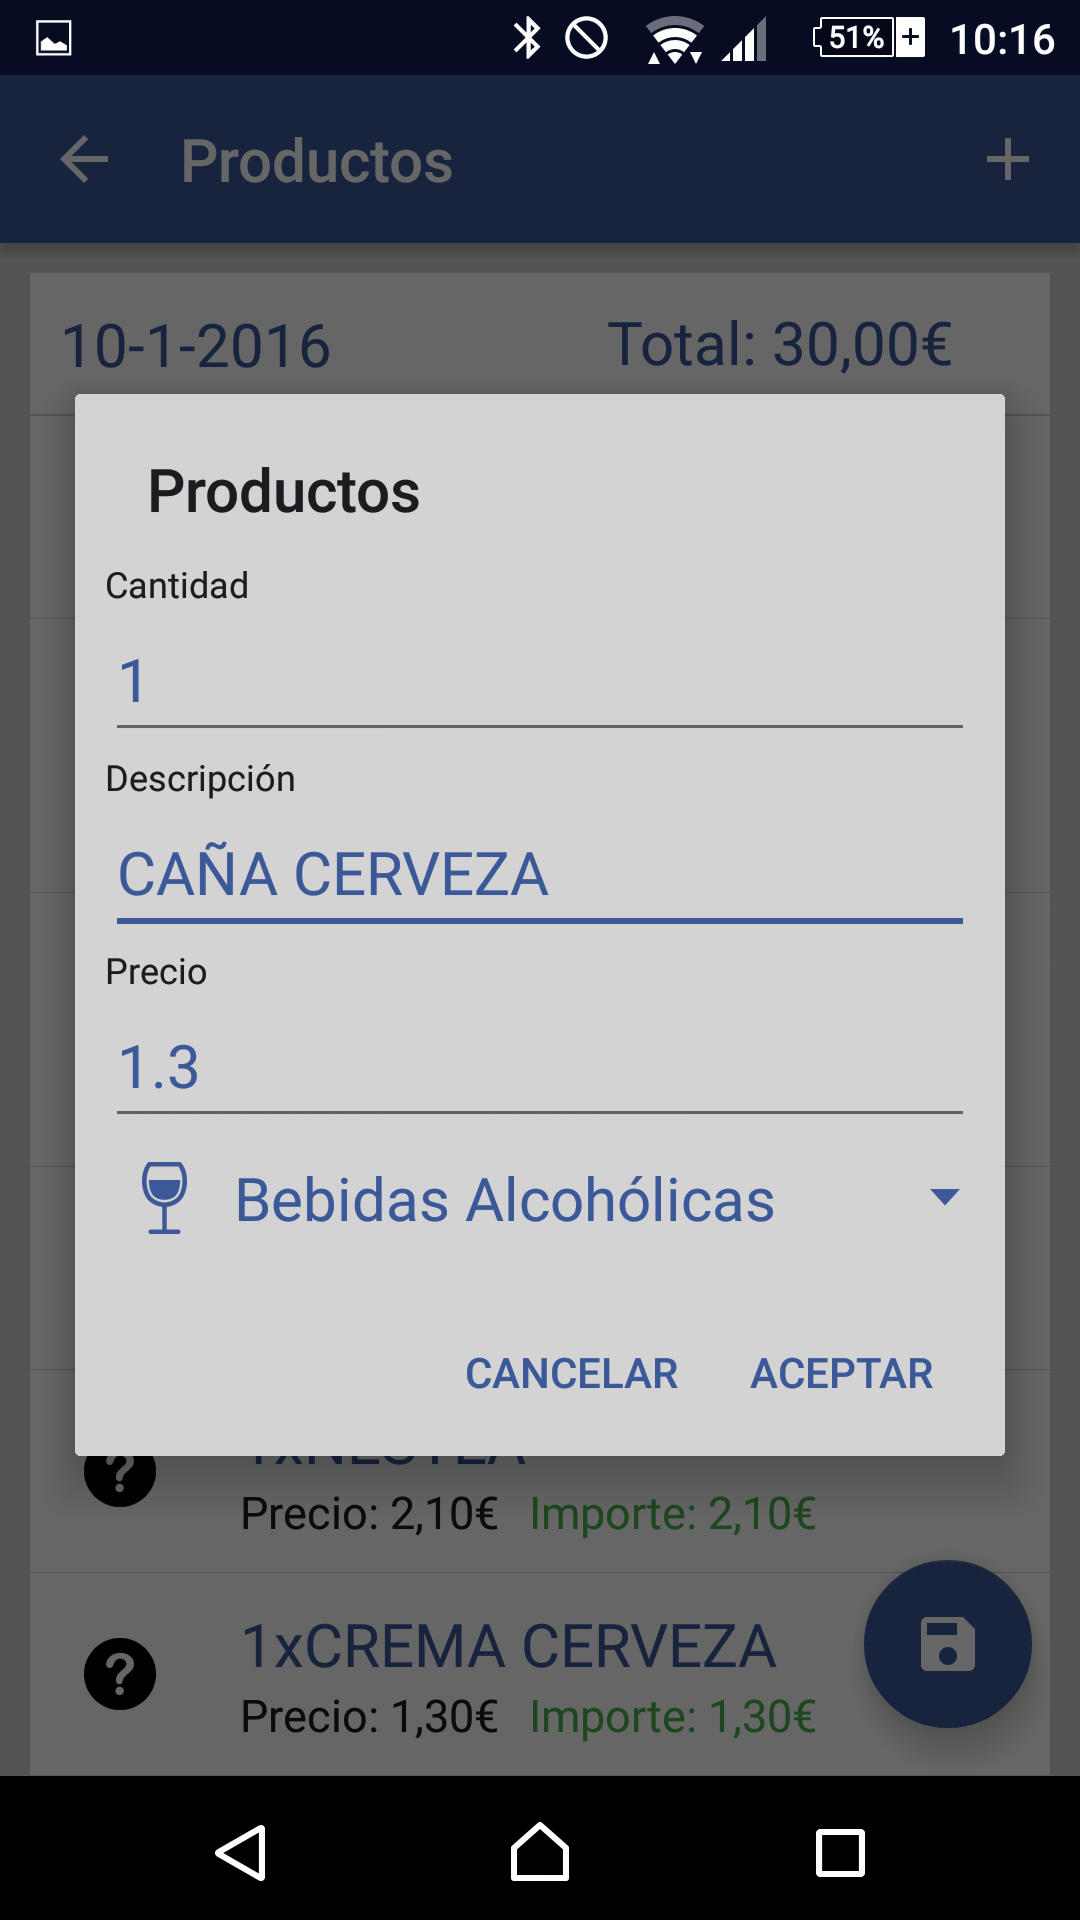
\includegraphics[width=\linewidth]{dialogoEdicion.png}
  \caption{Edición de un producto.}\label{fig:dialogoEdicion}
\endminipage
\end{figure}
\begin{figure}[ht]
\begin{center}
\minipage{0.60\textwidth}%
  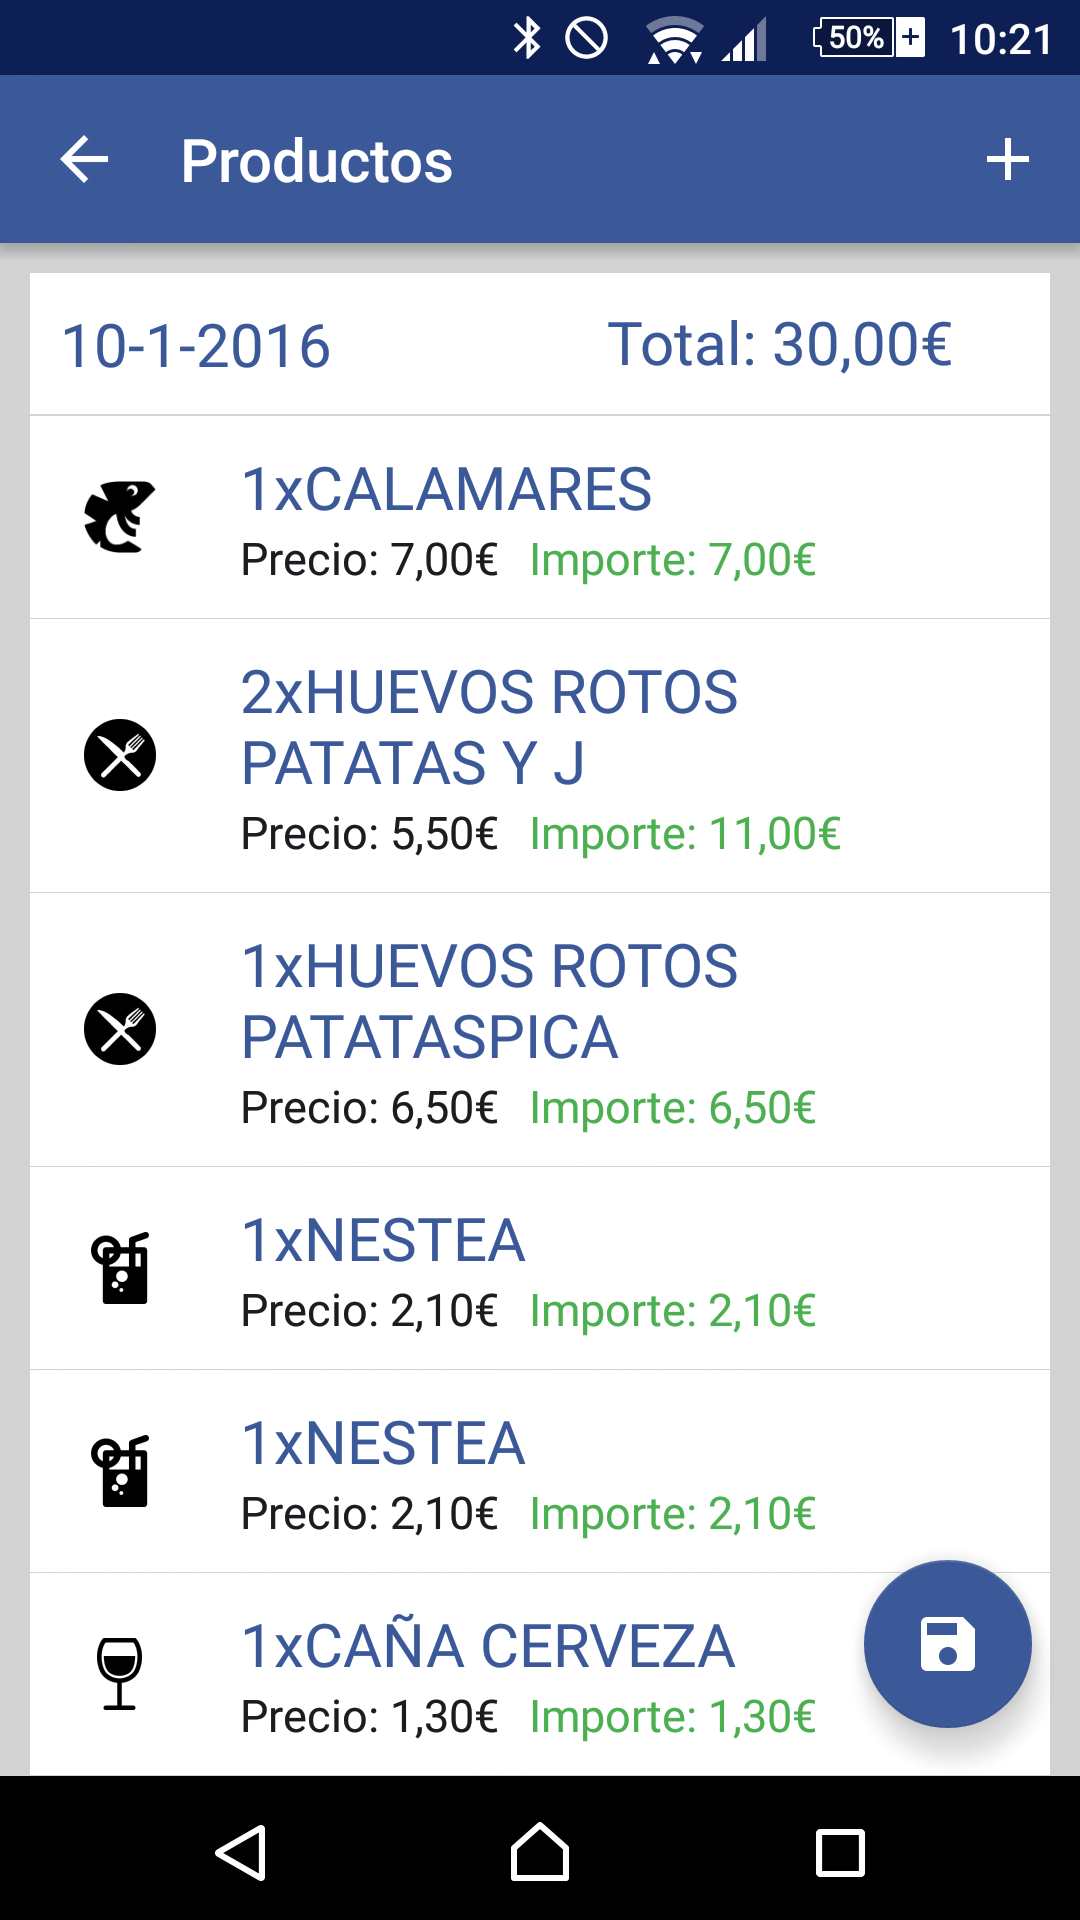
\includegraphics[width=\linewidth]{cargaCompleta.png}
  \caption{Proceso completado.}\label{fig:cargaCompleta}
\endminipage
\end{center} 
\end{figure}
\cleardoublepage
Cuando todos los productos sean correctos, pulsar en el botón \ref{fig:botonGuardar} para guardar, por el contrario si se desea añadir nuevos productos, hay que pulsar el botón \ref{fig:botonAnadir} situado en la esquina superior derecha, que se mostrará un diálogo similar al de edición(ver figura\ref{fig:dialogoEdicion}) para añadir un nuevo producto a la lista.

\begin{figure}[ht]
\begin{center} 
\minipage{0.32\textwidth}
  
\includegraphics[width=\linewidth]{botonGuardar.png}
  \caption{Guardar productos.}\label{fig:botonGuardar}
\endminipage\hfil
\minipage{0.32\textwidth}
  
\includegraphics[width=\linewidth]{botonAnadir.png}
  \caption{Añadir nuevo producto.}\label{fig:botonAnadir}
\endminipage
\end{center}
\end{figure}

\subsection{Vista de Resumen \label{resumen}}

Para ver el resumen de gastos se tiene  que pulsar la opción \textbf{Resumen} del menú de la aplicación(ver sección \ref{menu}).

En el gráfico se puede ver el gasto por categoría y el porcentaje sobre el gasto total que lleva el usuario acumulado.

\begin{figure}[ht]
\begin{center}
\minipage{0.60\textwidth}
  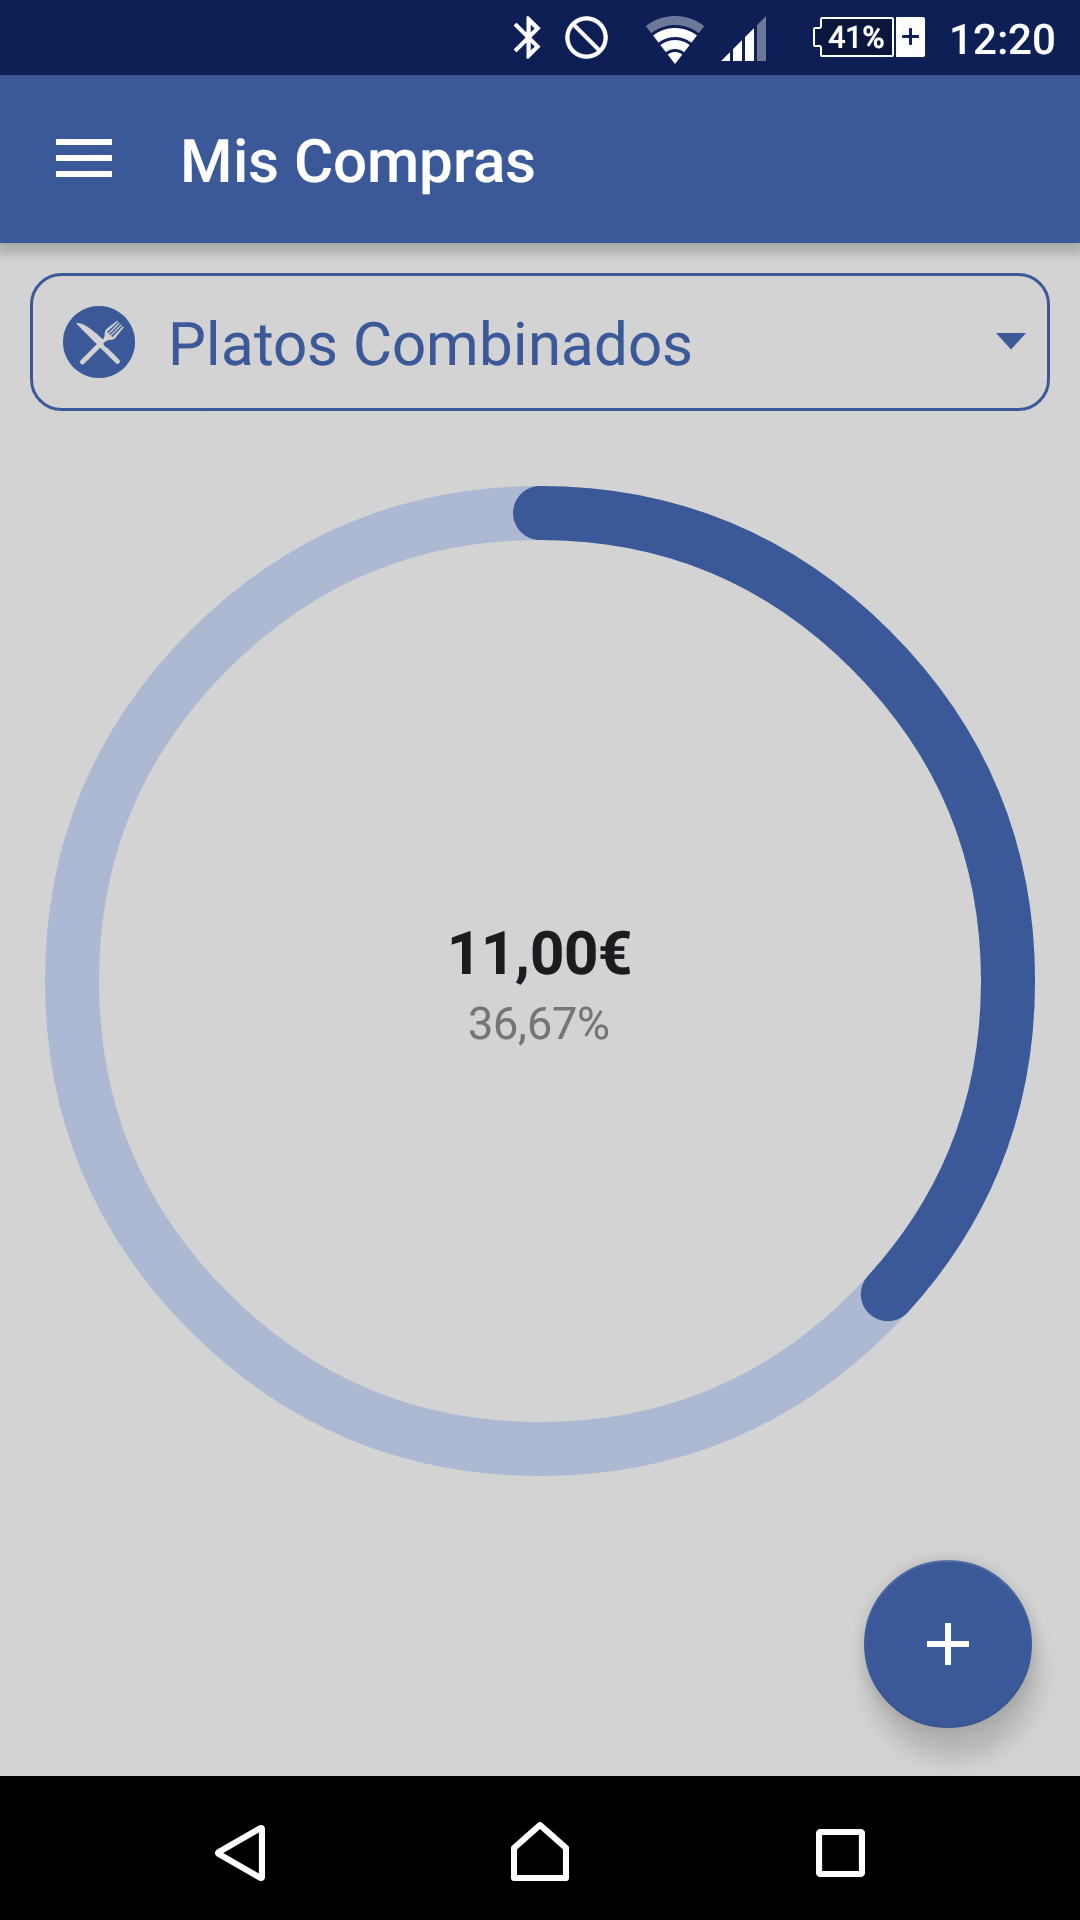
\includegraphics[width=\linewidth]{resumen.png}
  \caption{Vista de Resumen.}\label{fig:resumen}
\endminipage 
\end{center}
\end{figure} 

\cleardoublepage
\subsection{Consulta de Productos \label{consultaProdutos}}

Para consultar los productos adquiridos se tiene que pulsar la opción \textbf{Productos} del menú de la aplicación(ver sección \ref{menu}).

En la pantalla de Productos para realizar una consulta basta con pulsar el botón con el icono de lupa(ver figura \ref{fig:botonBusqueda}). 

\begin{figure}[ht]
\begin{center}
\minipage{0.32\textwidth}
  
\includegraphics[width=\linewidth]{botonBusqueda.png}
  \caption{Botón  de bisqueda.}\label{fig:botonBusqueda}
\endminipage
\end{center}
\end{figure}

Para realizar diferentes consultas se puede cambiar entre varias opciones, para poder cambiar los filtros de búsqueda se tiene que pulsar el botón de menú, situado en la esquina superior derecha de la pantalla y seleccionar la opción de filtros.

\imagen{opcionFiltros}{Filtro de productos.}

Cuando se pulsa en este botón, aparece un diálogo de selección del filtro deseado(ver figura \ref{fig:filtrosProducto} ), siendo estos \textbf{Fechas, Precio Unitario, Categoría}
\begin{itemize}
	\item \textbf{Fecha: }Fecha de compra del producto.
	\item\textbf{Precio Unitario: }Precio del producto.
	\item \textbf{Categoría: } Categoría del producto.
\end{itemize} Cuando se seleccione otro filtro, este cambia en la pantalla principal (ver figuras \ref{fig:filtroFechas}, \ref{fig:filtroPrecios} y \ref{fig:filtroCategorias}).



\begin{figure}[ht]
\begin{center}
\minipage{0.45\textwidth}
  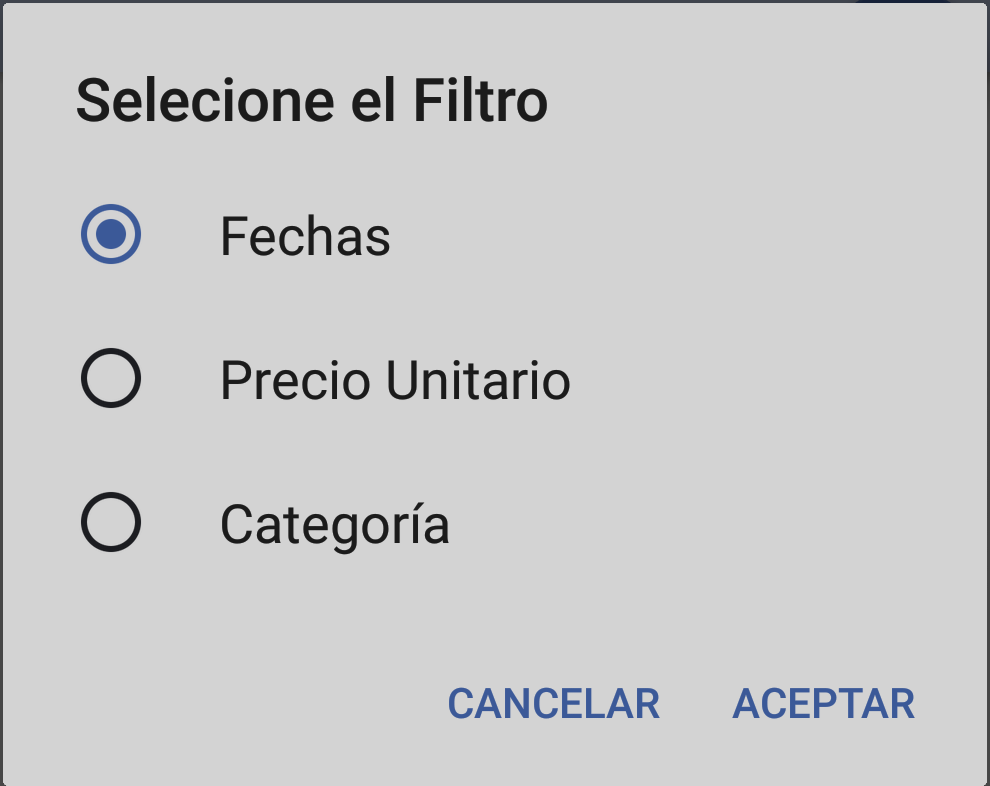
\includegraphics[width=\linewidth]{filtrosProducto.png}
  \caption{Filtros de busqueda de productos}\label{fig:filtrosProducto}
\endminipage
\end{center}
\end{figure}

\begin{figure}[ht]
\begin{center}
\minipage{0.60\textwidth}
  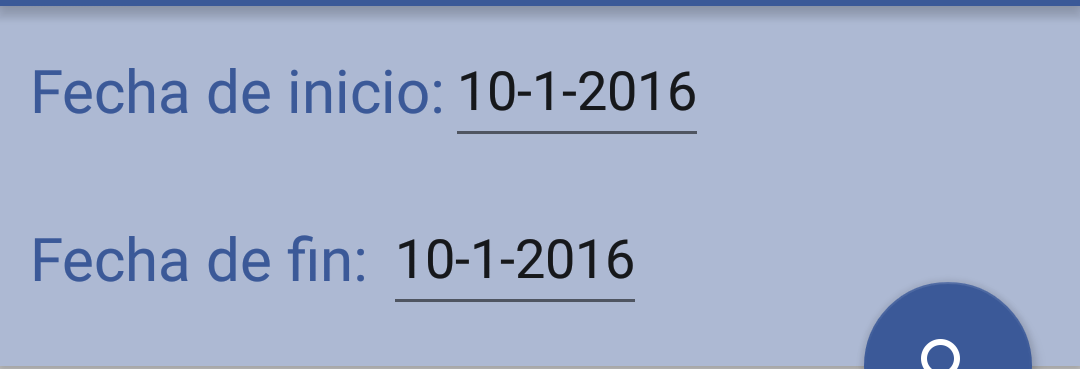
\includegraphics[width=\linewidth]{filtroFechas.png}
  \caption{Filtro por fechas.}\label{fig:filtroFechas}
\endminipage 
\end{center}
\end{figure}

\begin{figure}[ht]
\begin{center}
\minipage{0.60\textwidth}
  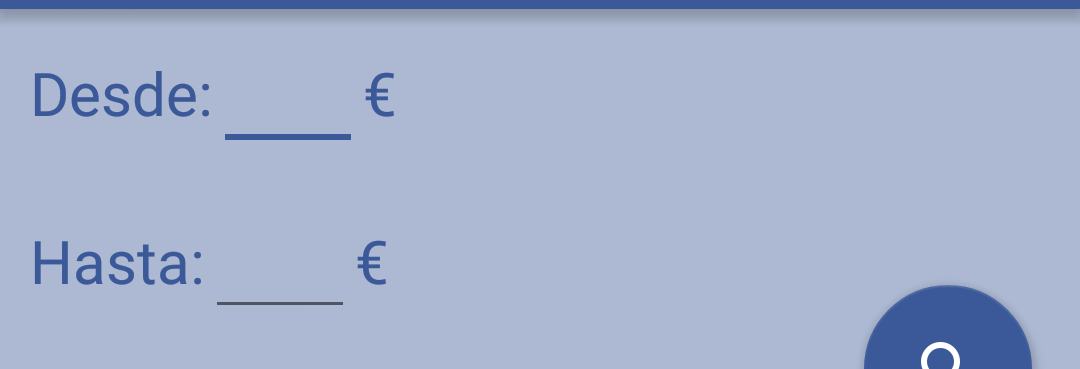
\includegraphics[width=\linewidth]{filtroPrecios.png}
  \caption{Filtro por precios.}\label{fig:filtroPrecios}
\endminipage 
\end{center}
\end{figure}

\begin{figure}[ht]
\begin{center}
\minipage{0.60\textwidth}
  \includegraphics[width=\linewidth]{filtroCategorias.png}
  \caption{Filtro por categorías.}\label{fig:filtroCategorias}
\endminipage 
\end{center}
\end{figure}
\cleardoublepage
Una vez seleccionado el filtro deseado y rellenado correctamente, al pulsar el botón de búsqueda(ver figura \ref{fig:botonBusqueda}) se muestra una lista de productos que cumplen el filtro seleccionado.

\begin{figure}[ht]
\begin{center}
\minipage{0.60\textwidth}
  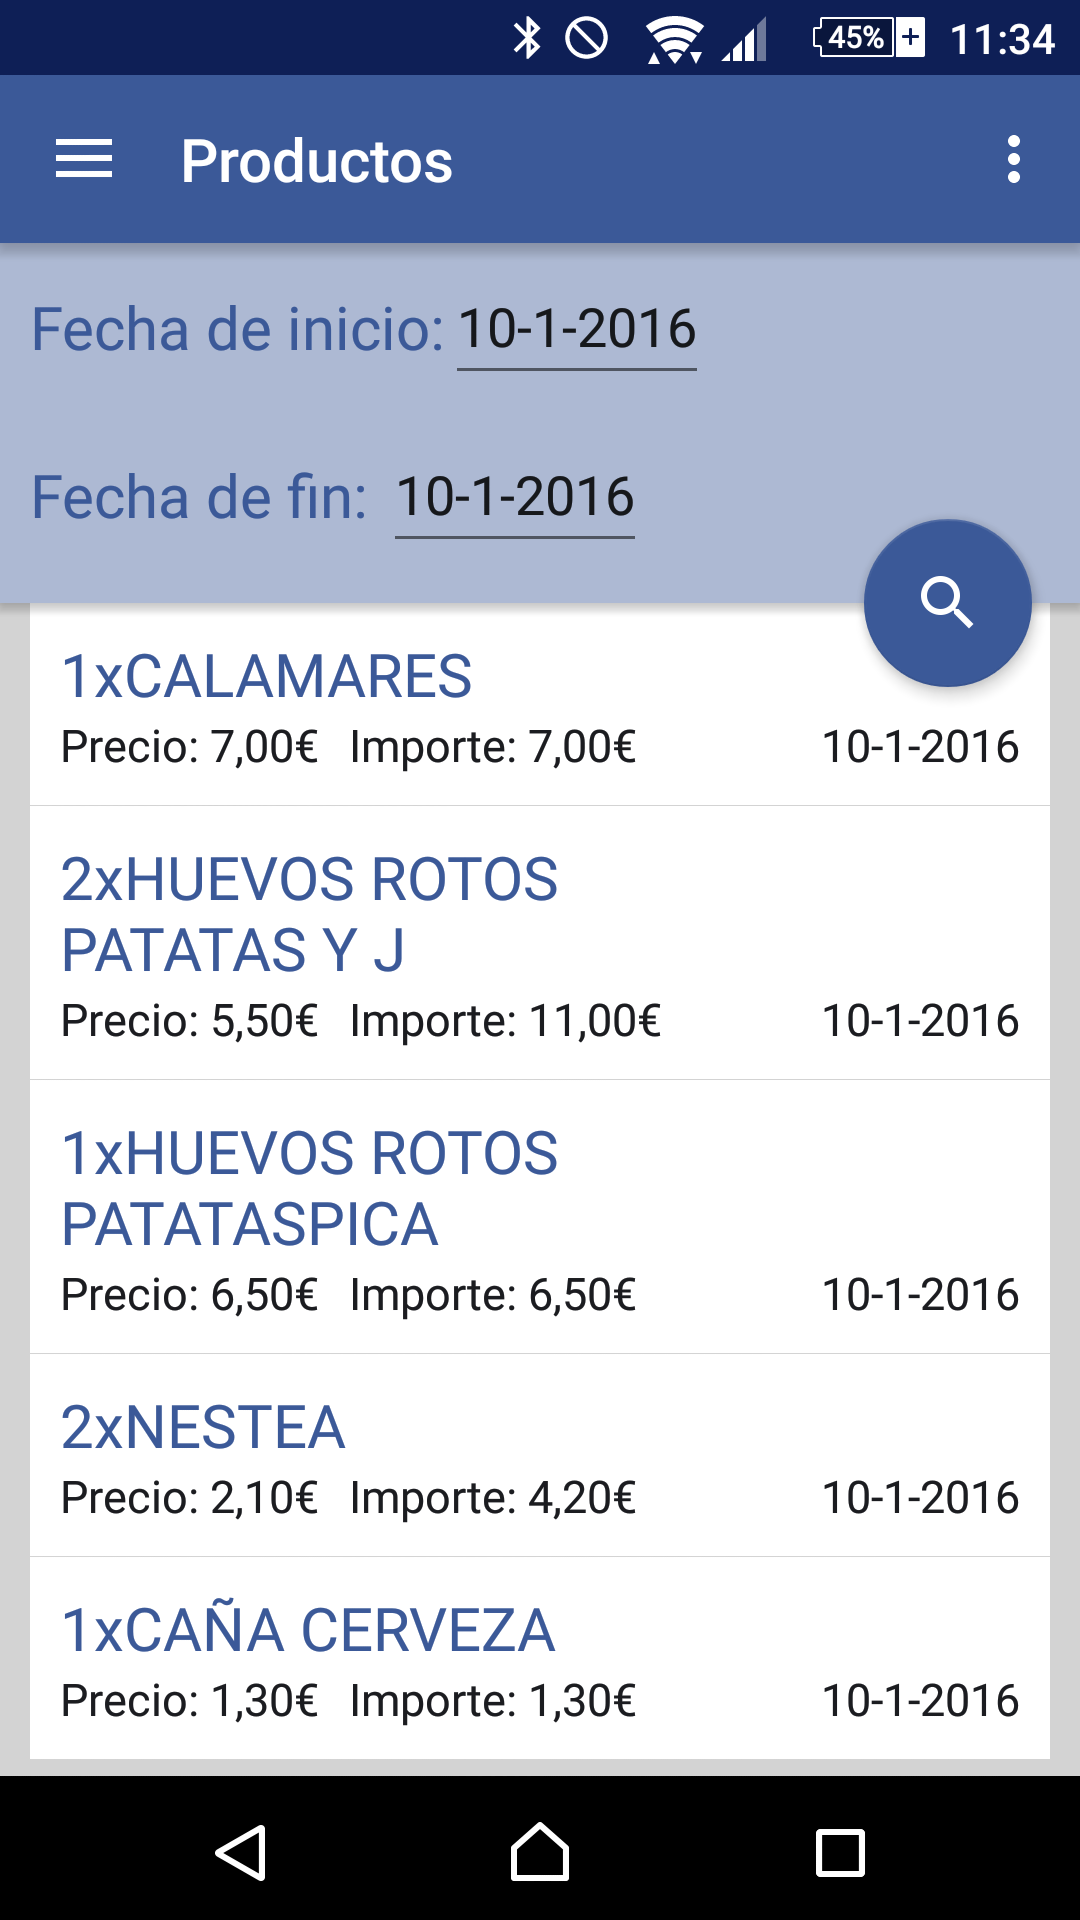
\includegraphics[width=\linewidth]{listaProductos.png}
  \caption{Ejemplo de lista de productos.}\label{fig:listaProductos}
\endminipage 
\end{center}
\end{figure}

\cleardoublepage

\subsection{Consulta de Compras \label{consultaCompras}} 

Para consultar las compras se tiene que pulsar la opción \textbf{Compras} del menú de la aplicación(ver sección \ref{menu}).

El proceso de consulta de compras es igual que en la consulta de productos(ver sección\ref{consultaProdutos}). Al terminar de realizar las consultas se obtiene una lista con las compras que cumplan los requisitos del filtro.
\begin{figure}[ht]
\begin{center}
\minipage{0.60\textwidth}
  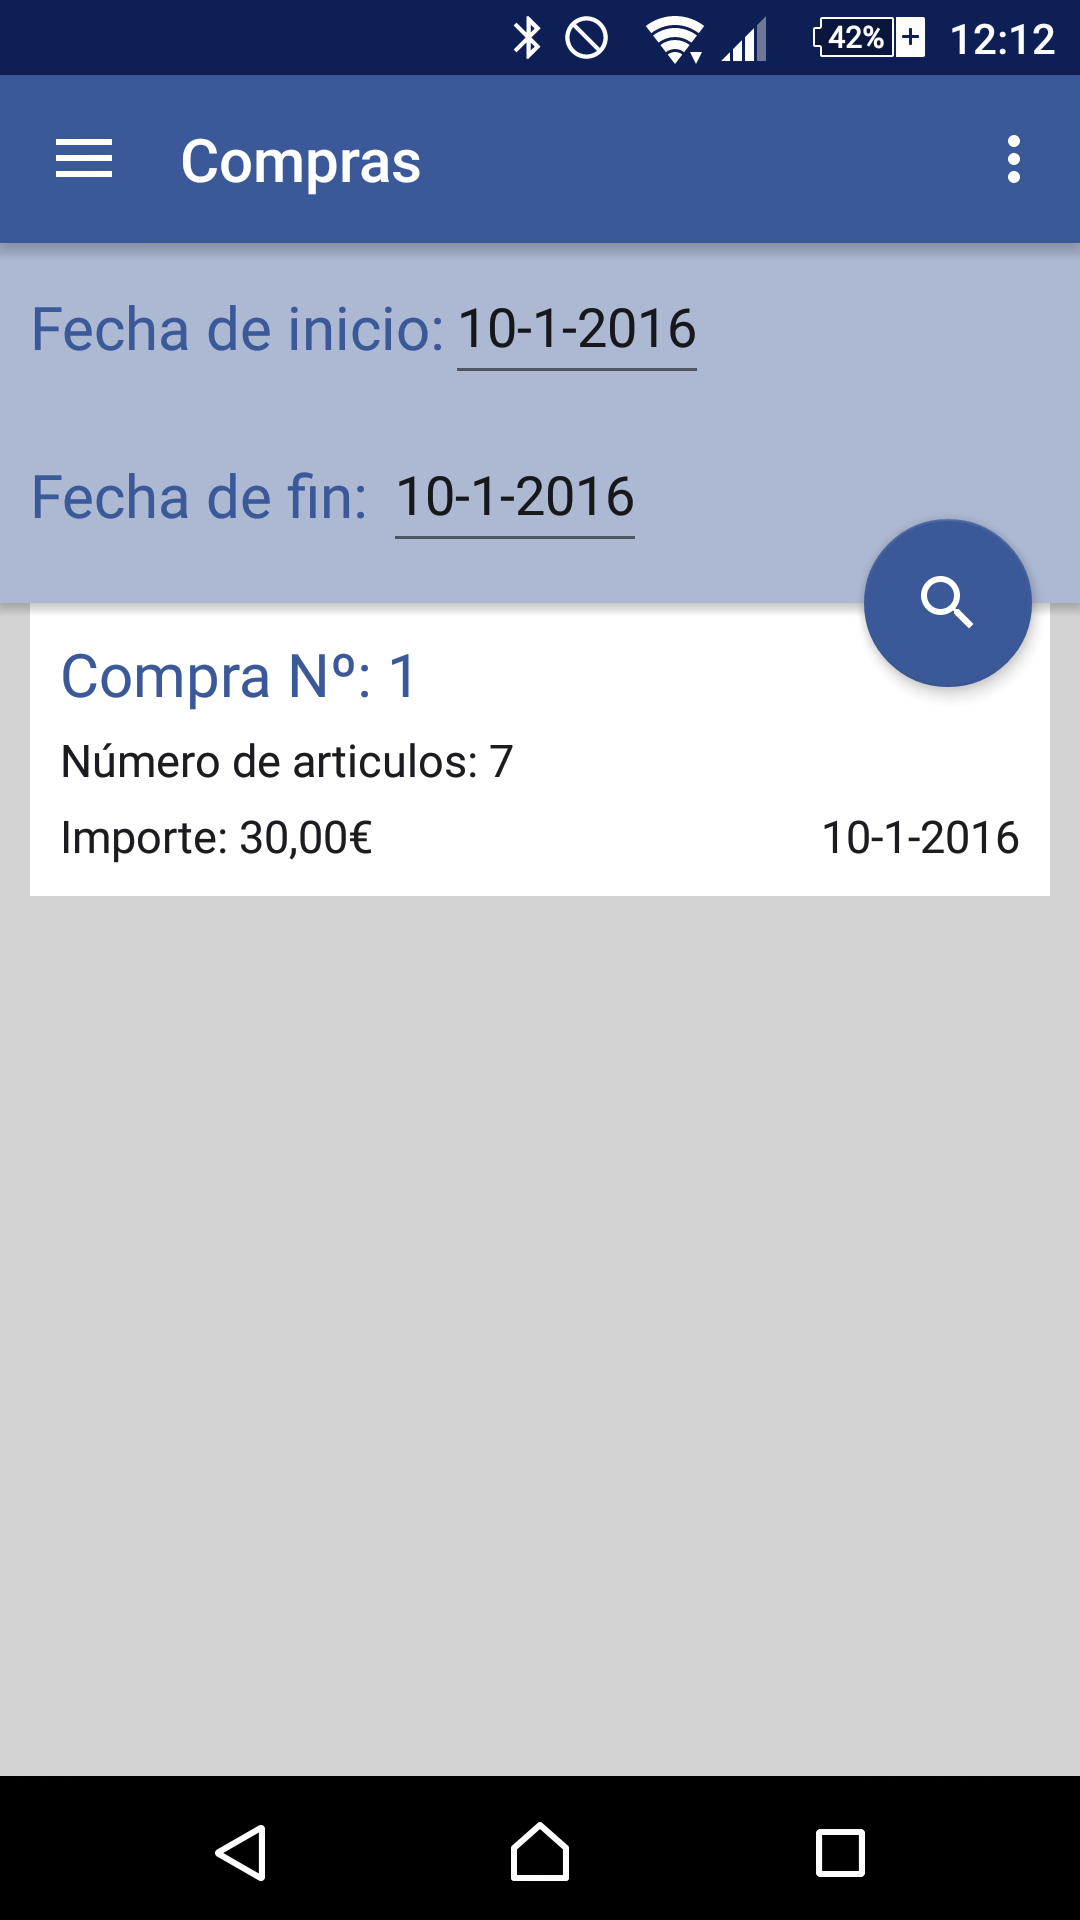
\includegraphics[width=\linewidth]{listaCompras.png}
  \caption{Ejemplo lista de compras.}\label{fig:listaCompras}
\endminipage 
\end{center}
\end{figure}

En este caso los filtros son:
\begin{itemize}
	\item \textbf{Fecha: }Fecha de compra.
	\item\textbf{Importe: }Importe de la compra.
\end{itemize}

Si se pulsa sobre un elemento de la lista, se cambia a una vista de detalle de los productos adquiridos en la compra seleccionada compra(ver figura \ref{fig:detalleTique}).

\begin{figure}[ht]
\begin{center}
\minipage{0.60\textwidth}
  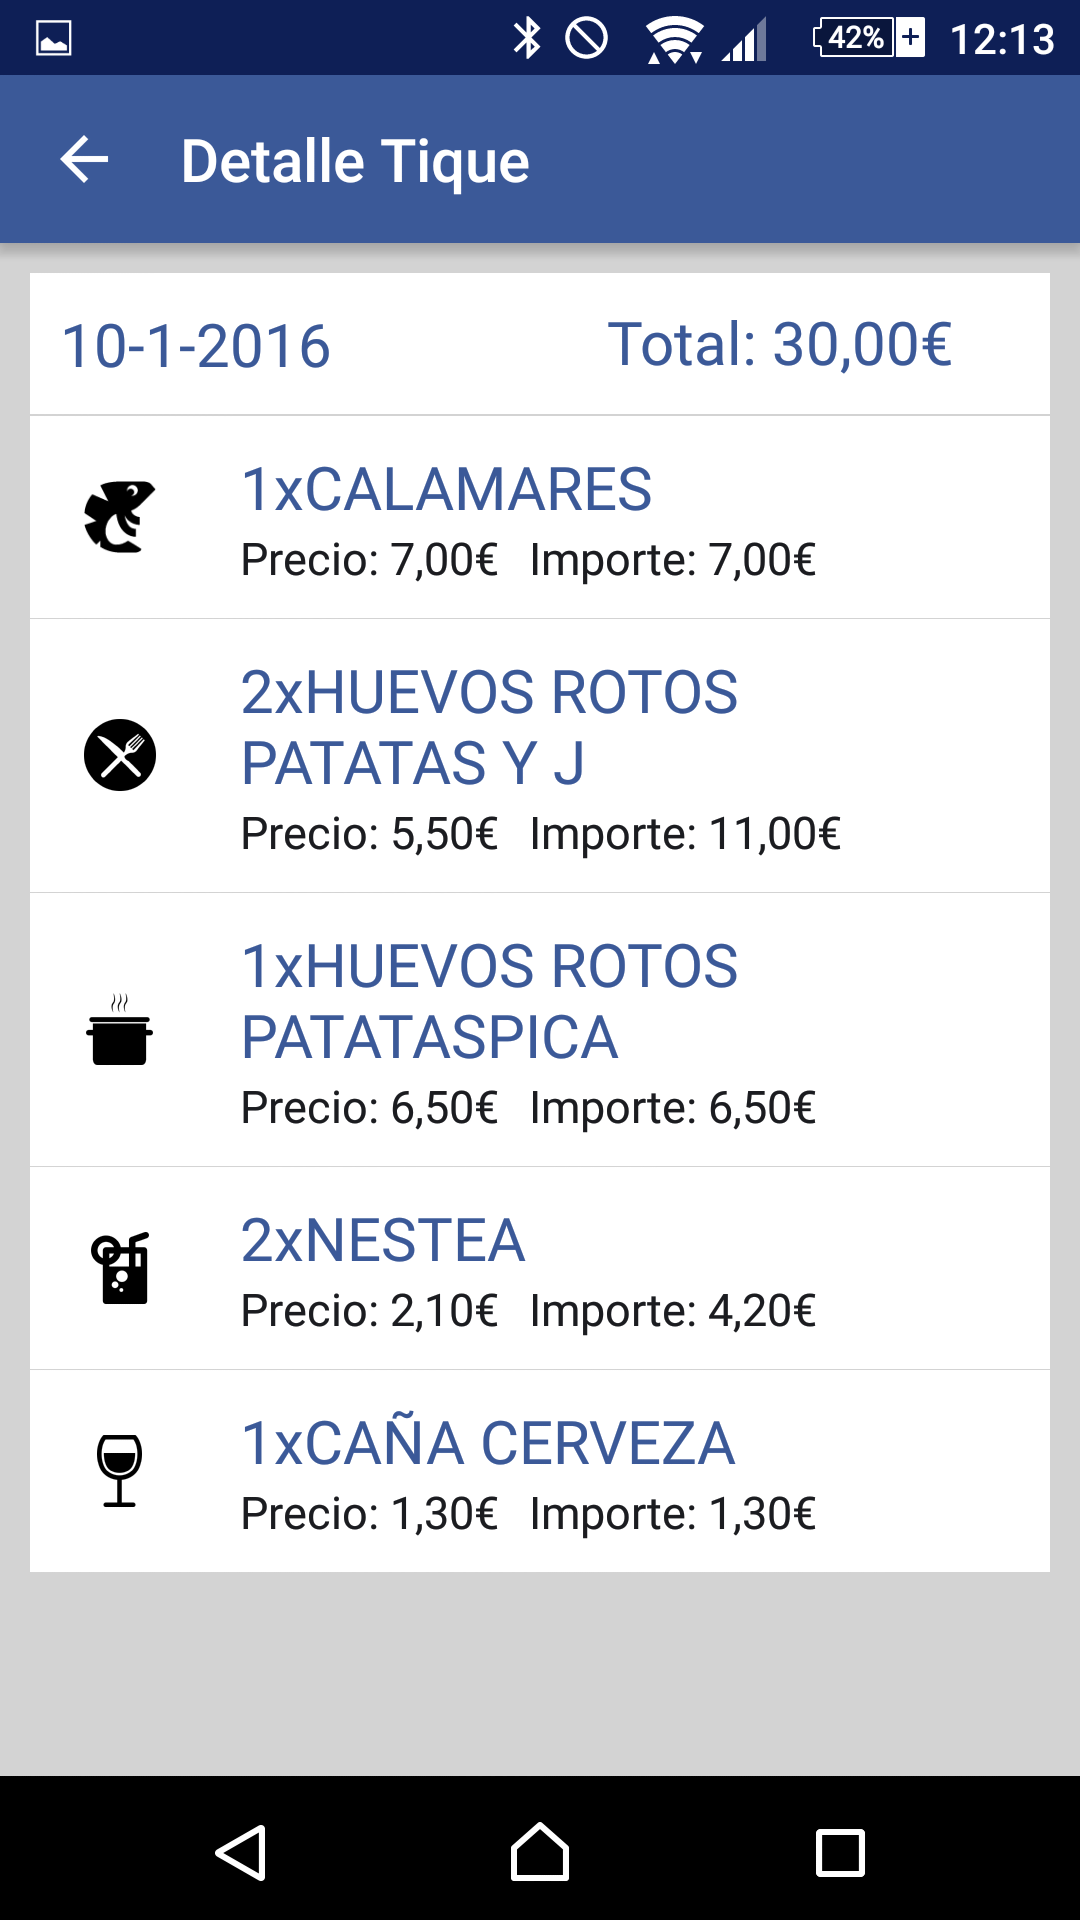
\includegraphics[width=\linewidth]{detalleTique.png}
  \caption{Vista de detalle de una compra.}\label{fig:detalleTique}
\endminipage 
\end{center}
\end{figure}